% !TeX spellcheck = en_US
\documentclass[10pt,a4paper, notitlepage]{report}
\usepackage[english]{babel}
\usepackage[latin1]{inputenc}
\usepackage{amsmath}
\usepackage{amsfonts}
\usepackage{amssymb}
\usepackage{epstopdf}
\usepackage{graphicx}
\usepackage{hyperref}
\usepackage{svg}
\usepackage{float}
\usepackage{lettrine}


\newcommand{\superref}[3]{\hyperref[#1]{#2} (\capitalisewords{#3} \ref{#1})}


\title{Design and development of \\ a long-range SLAM system}
\author{Irvin Aloise}


\begin{document}
\maketitle


\textbf{Keywords.} \textit{Mobile Robotics, SLAM, Computer Vision, Perception, Optimization}


\section*{Summary of Proposal}
Mobile robots, in order to accomplish tasks in the real world, need to be aware of where their own pose with respect to the world. This involves two things: the robot must have a \textit{map} of the environment and it must \textit{locate} itself inside of the created map. In robotics, the task of learning maps under pose uncertainty is called \textit{Simultaneous Localization and Mapping} (SLAM). SLAM systems are used in many applications, for example, \textit{industrial and service robotics}, \textit{space exploration} or \textit{autonomous cars}. 

\begin{figure}[h]
    \centering
    \resizebox{0.8\textwidth}{!}{\input{media/inkscape/graph_slam.pdf_tex}}
    \caption{A generic \textit{factor graph}: circles represent \textit{nodes} - poses in orange and landmarks in green -  while squares are \textit{edges} - pose edges are $u$-labeled while point edges are $z$-labeled. $u_4$ represents a \textit{loop-closure}.}
    \label{fig:graph}
\end{figure}

The robotics community has focused its efforts in this task since many years, and various approaches have been exploited. One of the most intuitive (and also effective) is the so called \textit{graph-based SLAM}\cite{lu1997globally}, in which the robot builds an hyper-graph where nodes represent its poses and interesting world points (landmarks), while the hyper-edges encode sensor measurements between a subset of nodes, as depicted in Figure \ref{fig:graph}. Graph-based SLAM systems have two main components: a \textit{front-end} that exploits sensors measurements to build the graph and a \textit{back-end} that performs non-linear optimization of the graph - as shown in Figure \ref{fig:slam-overview}. 

Even if research in robotics has done several steps forward, the SLAM problem is not solved. Lots of questions are still open and many issues are largely unexplored \cite{carlone2016slam-survey}. One of these open problems is the fact that current state-of-the-art systems are not scalable. 

\textit{Scalability} is a key component to build robots able to cope with real-world and long-range tasks. Examples can be found in \textit{Precision Agriculture} - e.g. a drone that has to map several huge fields to track plant growth - or in \textit{Autonomous Driving Vehicles} - e.g. a fleet of self-driving trucks that deliver stuff ordered on the Internet to the clients - and in many others fields. The graph of current state-of-the-art can \textit{grow unbounded} for long-range tasks, making impossible real-time optimization and saturating robots resources, causing a certain failure of the system. Even storing the map becomes a problem when dimensions start to grow.

Another problem comes from the \textit{map}: for long-range tasks, we know that maps can be very big in space and time, but how do we scale them in order to keep them still usable? Moreover, the way in which a map is intended must be revised, to obtain a fully scalable system: generally, we know that maps are a \textit{collection of interesting points} obtained by the processing of sensors' data, stored \textit{locally} in the robot. \textit{But what if the map is in the environment}? What if a robot can enter in a place and download data on the environment, updating it while executing its other tasks? In this way, maps can be more complex and contain more useful information in order to understand the environment - e.g. objects' position, road signals, warnings and so on. Taking people as example, the precise planimetry of a park is not useful in terms of knowledge and it represents a complex object to read and remember, while a simple sketch of the park that emphasizes entrances and exits, points of interests and walkable paths is very powerful and allow us to do what we want in the park. What if environmental information can be represented like this also in robotics? If this would be the case, maps will be smaller, lighter and more informative. Thus, this decentralized and content-aware map representations are essential for scalability and represent a step forward for cognitive robots that do not just sense the environment, but that understand it. 

\vspace{10px}

Given all those premises, what I expect to obtain in my research is a system designed to deliver state-of-the-art performances even after several hours of usage, proposing a way to efficiently perform back-end optimization together with new map representations that can deal with huge environments, opening to new research paths in the involved fields.

\begin{figure}
    \centering
%    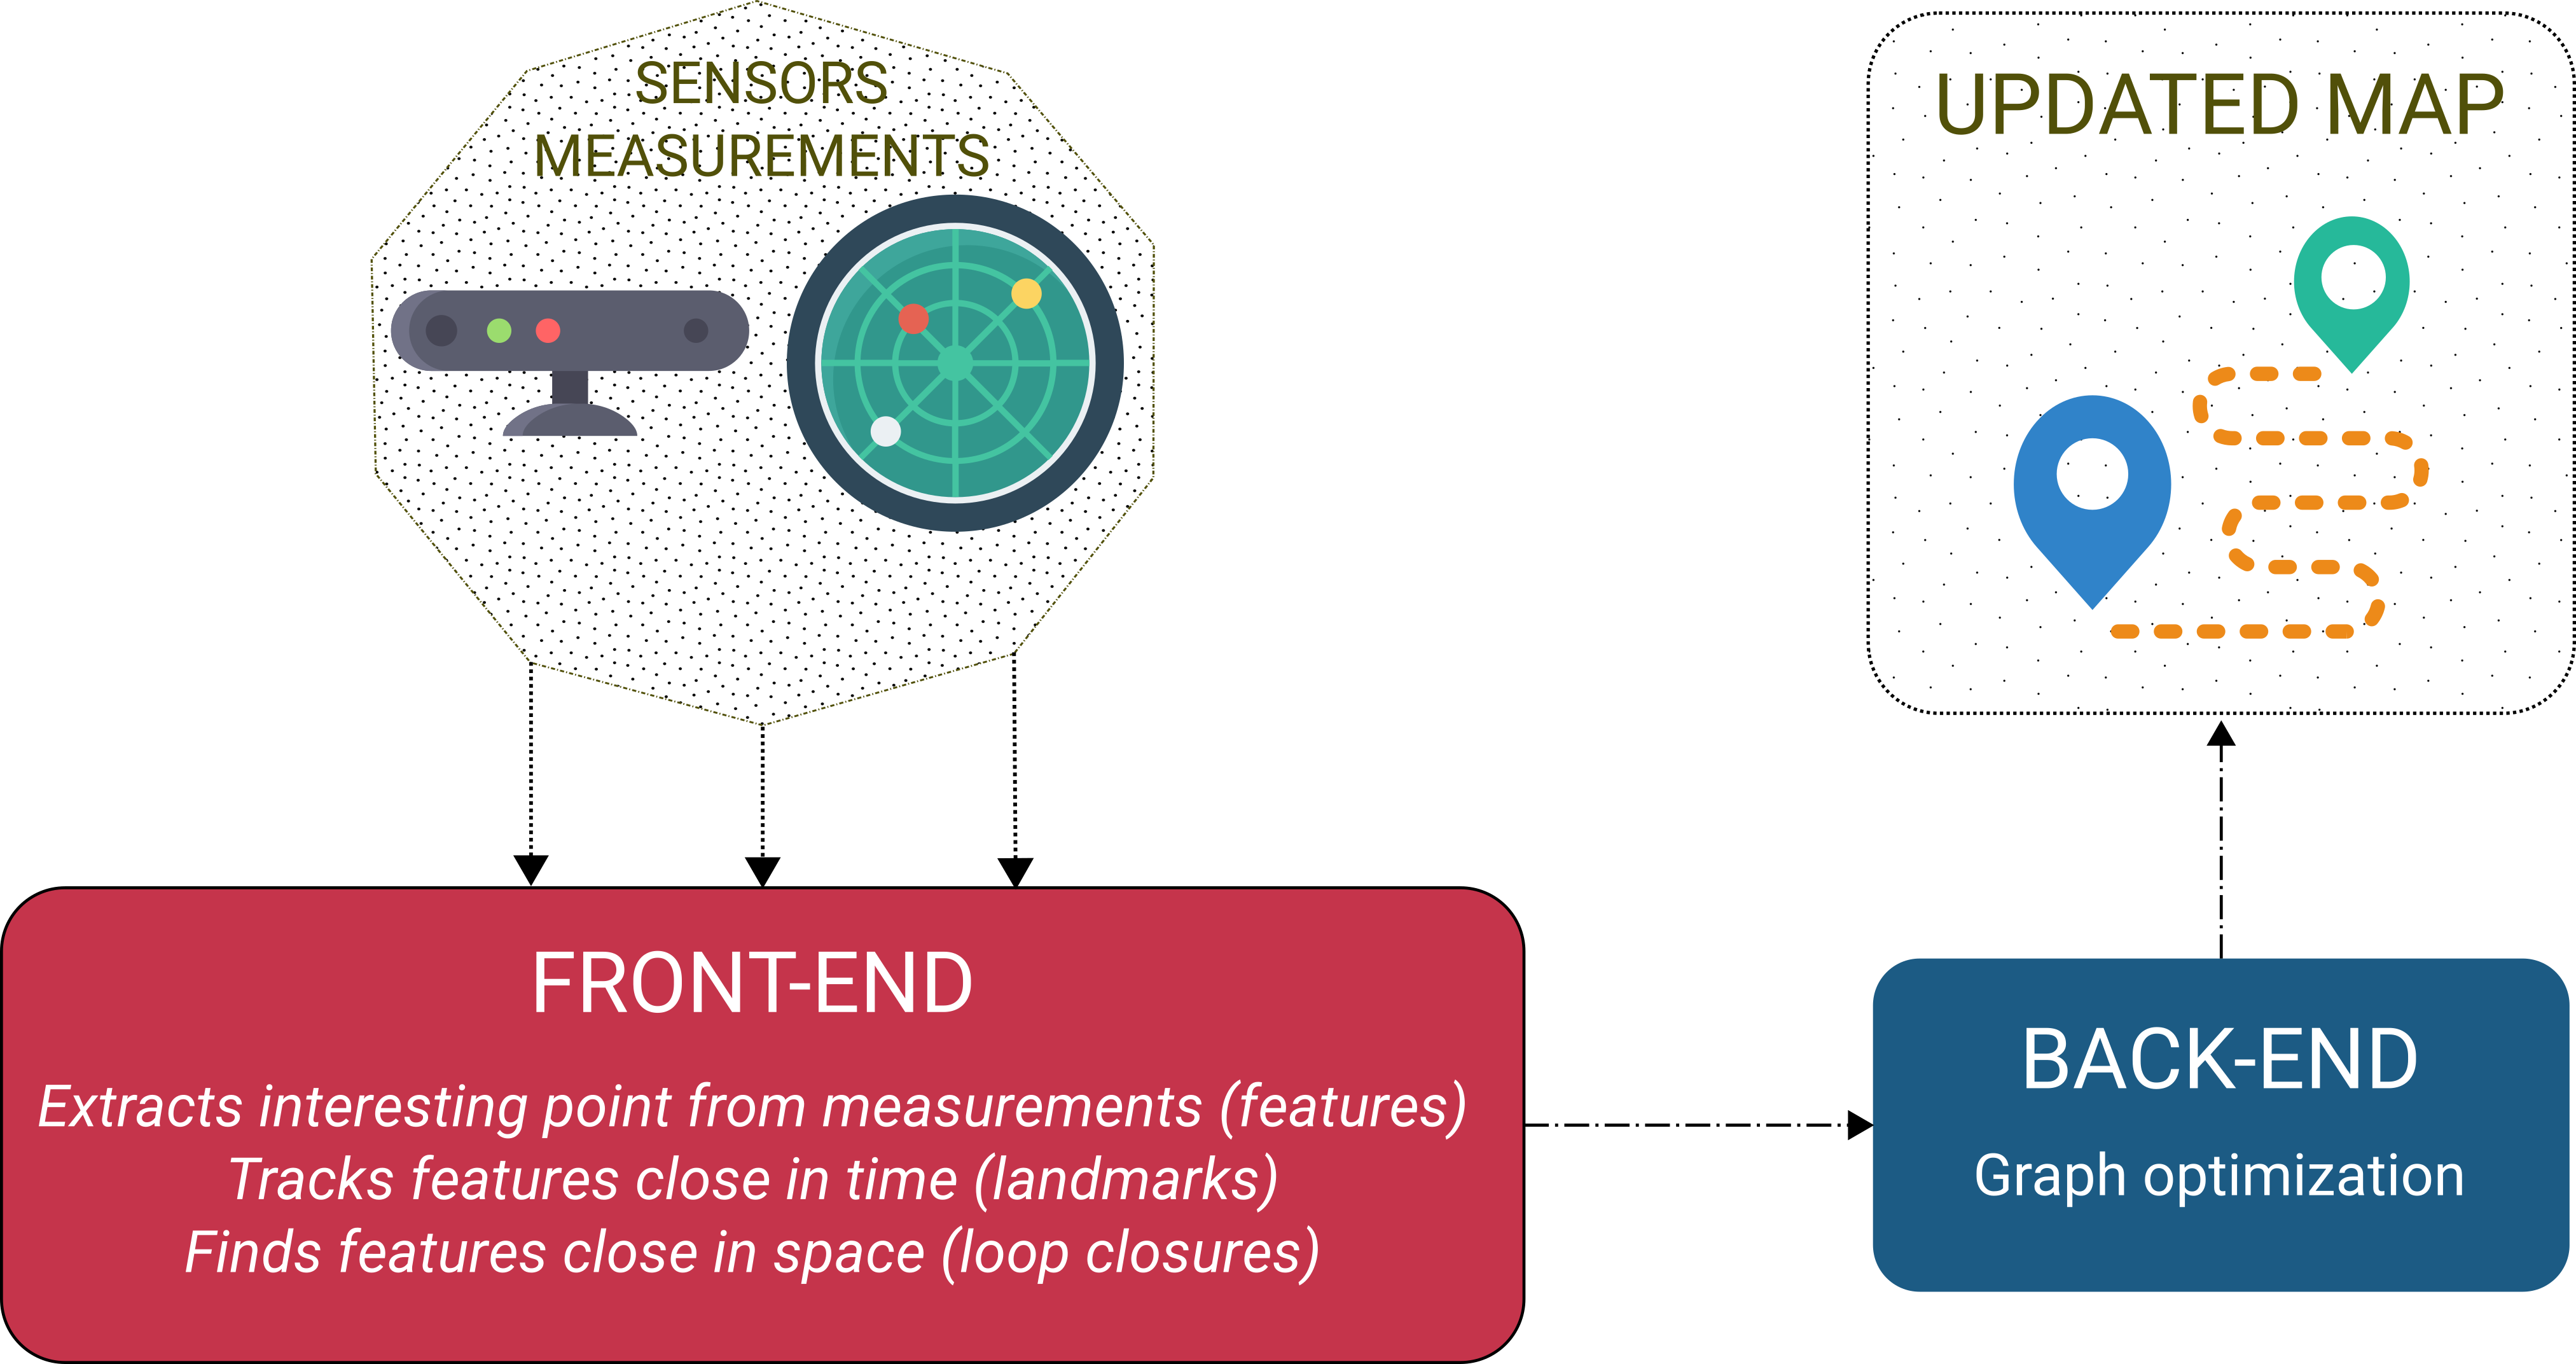
\includegraphics[width=0.9\linewidth]{media/inkscape/slam_system_mod.png}
    \resizebox{0.8\textwidth}{!}{\input{media/inkscape/slam_system_mod.pdf_tex}}
    \caption{SLAM system overview: sensor measurements are fed into the \textit{front-end}, that extracts features and solves the \textit{data-association}, building the graph that will constitute \textit{back-end's input}. At this point, \textit{Maximum A Posteriori} estimation is done and the map is updated.}
    \label{fig:slam-overview}
\end{figure}


\section*{State of the Art}
In Robotics, an autonomous agent performs Simultaneous Localization and Mapping (SLAM) when it builds a map of the environment using different kind of sensors while localizing itself in the created map. Its core is a complex non-linear mathematical problem and it has been studied since 80s \cite{durrant2006simultaneous} \cite{bailey2006simultaneous}; during this early stage, statistical basis that will constitute SLAM's core were investigated. Only in late 90s probabilistic approaches started to spread, mainly based on \textit{Extended Kalman Filters} \cite{leonard1990dynamic} \cite{dissanayake2001solution} and \textit{Expectation Maximization} algorithms \cite{dellaert2003mcmc} \cite{thrun2001probabilistic}. Filtering continued to gain popularity with \textit{Particle Filters} - employed in the remarkable work of \textit{Montemerlo et al.} \cite{montemerlo2002fastslam} - and its future refinements, like \textit{Rao-Blackwellized Particle Filters} \cite{grisetti2005improving} \cite{carlone2010rao} \cite{tipaldi2007heterogeneous}.

Filtering-based approaches bring multiple drawbacks, like low computational efficiency and low accuracy due to problem's high nonlinearities; for these reasons, \textit{Maximum A Posteriori} (MAP) algorithms started to gain popularity and a step back to the solution of Lu \textit{et al.} \cite{lu1997globally} has been done. Exploiting more powerful computing resources, the problem can be formalized as an \textit{hyper-graph} where each node represents a robot pose or a landmark - a point of interest placed in the robot's surrounding - and each hyper-edge represents a constraint between a subset of nodes. 

Exploiting graph's topology, factor-graph optimization can achieve impressive performances as stated in the works of Dallaert \textit{et al.} \cite{dellaert2006square} and Kummerle \textit{et al.}  \cite{kummerle2011g}. MAP optimizers \cite{kummerle2011g} \cite{dellaert2012gtsam} \cite{ceres-solver} \cite{kaess2012isam2} are able to easily deal with huge graph and incremental optimization, delivering state-of-the-art performances both in speed and accuracy terms.

While SLAM's back-end performs map optimization, graph population is done by system's front-end, exploiting sensors' measurements. State-of-the-art systems usually acquire data from cameras (RGB or RGB-D) or 3D-LiDARs. The former ones in particular are gaining much attention since they are cheap and can be mounted basically on every kind of robot - in single or stereo configurations. Current benchmark systems for \textit{monocular visual SLAM} are \textit{ORB-SLAM} \cite{mur2015orb-slam} and \textit{LSD-SLAM} \cite{engel2014lsd-slam}, while for \textit{stereo configurations} it is impossible to ignore \textit{ORB-SLAM2} \cite{mur2017orb-slam2}. The former and the latter systems rely on the extraction of visual features from the scene, making them vulnerable to light changes or untextured scenes. \textit{LSD-SLAM} instead uses raw visual data to track robot motion and, thus, it is more robust to such weakness at the cost of more computational power needed to deliver real-time performances.

All those systems - even if they are able to produce significant results in terms of accuracy and speed - share one big drawback: the \textit{lack of scalability} that would allow to deal with real-world scenarios. In this sense, the research community is still far from a solution, even if some early attempts are made. Possible approaches to scalability that can be found in literature are based on \textit{node - edge sparsification} \cite{kretzschmar2011graph-pruninig} \cite{huang2013consistent} - that consists in pruning less informative node or factors following a suitable criterion - \textit{parallelization of SLAM system} \cite{ni-dallaert2010nested-dissections} \cite{ni-dallaert2007tectonicSAM} \cite{grisetti2010hogman} or \textit{multi-robot SLAM} \cite{cunningham2013ddfSAM2} \cite{lazaro2013mr-slam}. All those approaches are too naive and still miss the point on long-term scalability issues like \textit{robustness}, the possibility to run with \textit{limited resources} and \textit{efficient data storage methods}. It is good to notice that a scalable SLAM system, besides all those features, has to operate in different environments, thus adaptation must be taken in consideration to avoid failures - e.g. map representation adaptation, system's parameters auto-tuning to different environmental conditions - but none of the existing SLAM system provides such competences.

\section*{Research Objectives}
Scalability is the first step towards \textit{long-range SLAM}, allowing the robot to operate for long periods without saturating system's resources. 

My research will focus on the development of a brand new SLAM system that can handle issues due to operations in large environments and for long continuous time. Scalability can be achieved at different level and, thus, there are several topics that I plan to cover during my research period.

Obviously, the first step is a deep review of the literature to better understand how state-of-the-art systems work and where modifications are needed to improve scalability. At this point, it is possible to active develop some novel approaches to accomplish the goal.

It has been demonstrated that using \textit{direct linear solvers}, factor-graphs grow quadratically with the number of variables; moreover, loop-closures cause a lessening of the problem's sparsity, leading to more computational-heavy optimization steps. With this in mind, \textit{graph efficiency} must by seriously improved in order to let the system run properly. \textit{Sub-graph partitioning} \cite{grisetti2012condensed-m} represents a good starting point to achieve results in this direction. For example, compress and off-load parts of the graph that are not relevant for the current state of the robot may lead to an easier optimization from a computational point of view. It is good to notice that this means to perform non-global optimization, thus, convergence's quality must be also take in consideration to avoid failures.

Major improvements may also come from more efficient map representations. Current systems rely on point-clouds or volumetric map but those methods waste a lot of memory - e.g. the representation of an empty room still need lots of resources to store all the landmarks found in it, even if that room is not relevant and does not contain useful informations. \textit{Compressing known part of the map} \cite{lynen2015getoutofmylab} can represent the base on which start more detailed analysis. A possible approach may be \textit{map decentralization}, where buildings - or generic areas - hold their own map. In this way the robot can simply load the map, perform its task while updating missing parts - or modifications - of the downloaded map and, finally, upload the new representation freeing its own resources employed to locally store it. In this way even less powerful robots can be used for autonomous long-range tasks. More efficient maps can be obtained using \textit{high-level representations}, that would bring a deeper understanding of robots' surroundings. Speaking of recognition, it is impossible to not mention the results of \textit{Convolutional Neural Networks} \cite{krizhevsky2012alexnet} in such area. CNNs deliver state-of-the-art performances in object recognition and - even if they need long training time - may offer a big aid in building more expressive maps, starting also from point-cloud representations \cite{maturana2015voxnet}.

In order to have a functional out-of-the-box long-range mapping, it is required to design the system in a way that is able to deal with dramatic environmental changes - e.g. night-day shifts or indoor-outdoor transitions. Again, \textit{Machine Learning} techniques can come in aid, providing ways to overcome this issue - e.g. deploying a simple \textit{Artificial Neural Network} (ANN) that computes the right parameters which maximize the accuracy.

Finally, integrating all those features with a suitable SLAM front-end, I expect to deliver improved performances in terms of scalability for long-range mapping.

\section*{Results, impacts and benefits}
Simultaneous Localization and Mapping is far from being solved in lots of robotics instances. Many problems are still unsolved while other continue to arise, thus, the main purpose of my research consists in finding answers for some of those questions. 

A scalable robust SLAM system is required in many application, like \textit{Precision Agriculture} or \textit{Autonomous Driving Cars}. Robots operating in fields or highways have to run for many kilometers to accomplish a task, traversing different type of surroundings and facing dramatic changes in environmental conditions. Obviously, failures can come from multiple sources and must be solved to provide end-users fail-safe robots. Innovation in this field will bring to us more powerful agents capable of building and handling large-scale time-varying maps, allowing them to accomplish more complex tasks in a fully autonomous way. Thus, taking in consideration the question \textit{"Is scalable SLAM really needed?"}, of course the answer depends on the application, but, if we want to look at the future of robotics, then the answer is \textit{yes}.

Scalable SLAM is achieved combining powerful front-end with an efficient and smart back-end, building a map that is expressive but memory-thrifty. This means that succeeding in this purpose will bring major benefits to robotics community together with other related research fields - e.g. pure optimization theory, computer graphics and machine learning -  and will bring new challenges and opportunities for the SLAM community - e.g. the use Deep Learning. 

\vspace{5px}

Scalable SLAM - and robotics in general - is an important step towards real-world use of robots in daily situations. For this reason, what I do expect from my research is the creation of a system designed with those concepts in mind, that can be used in different situations without too much effort and that provides state-of-the-art accuracy, opening new paths for future investigations in such area.




\bibliographystyle{unsrt}
\bibliography{bibliography}

\end{document}